\newsec{Assorbimento dei raggi X}

\subsection{Verifica di Lambert-Beer}

Per verificare la legge di Lambert-Beer \cref{eq:lambertbeer}, studiamo l'assorbimento dei raggi X da parte di vari spessori di alluminio.
Gli spessori che abbiamo utilizzato e le relavtive frequenze sono riportate in tabella:

\begin{table}[]
  \centering
  \tiny
  \begin{tabular}{cc|cc}
    \hline
    $x [mm]$ & $\delta x [mm]$ & $ 
    u [s^{-1}]$ & $\delta  
    u [s^{-1}]$ \\
    \hline
    3.50 & 0.05 & 5.7 & 0.5\\
    3.00 & 0.05 & 10.9 & 0.7\\
    2.50 & 0.05 & 13.4 & 0.8\\
    2.00 & 0.05 & 18.6 & 1.0\\
    1.75 & 0.05 & 20.7 & 1.0\\
    1.60 & 0.05 & 23.2 & 1.1\\
    1.50 & 0.05 & 24.9 & 1.1\\
    1.35 & 0.05 & 31.5 & 1.3\\
    1.25 & 0.05 & 31.7 & 1.3\\
    1.10 & 0.05 & 38.1 & 1.4\\
    1.00 & 0.05 & 41.2 & 1.4\\
    0.85 & 0.05 & 48.4 & 1.6\\
    0.75 & 0.05 & 60.5 & 1.7\\
    0.60 & 0.06 & 69.2 & 1.9\\
    0.50 & 0.05 & 83 & 2\\
    0.35 & 0.03 & 120 & 2\\
    0.25 & 0.03 & 199 & 3\\
    0.100 & 0.010 & 574 & 5\\ 
    0.0 & 0.0 & 1592 & 9
  \end{tabular}
\end{table}

\begin{figure}[]
    \centering
    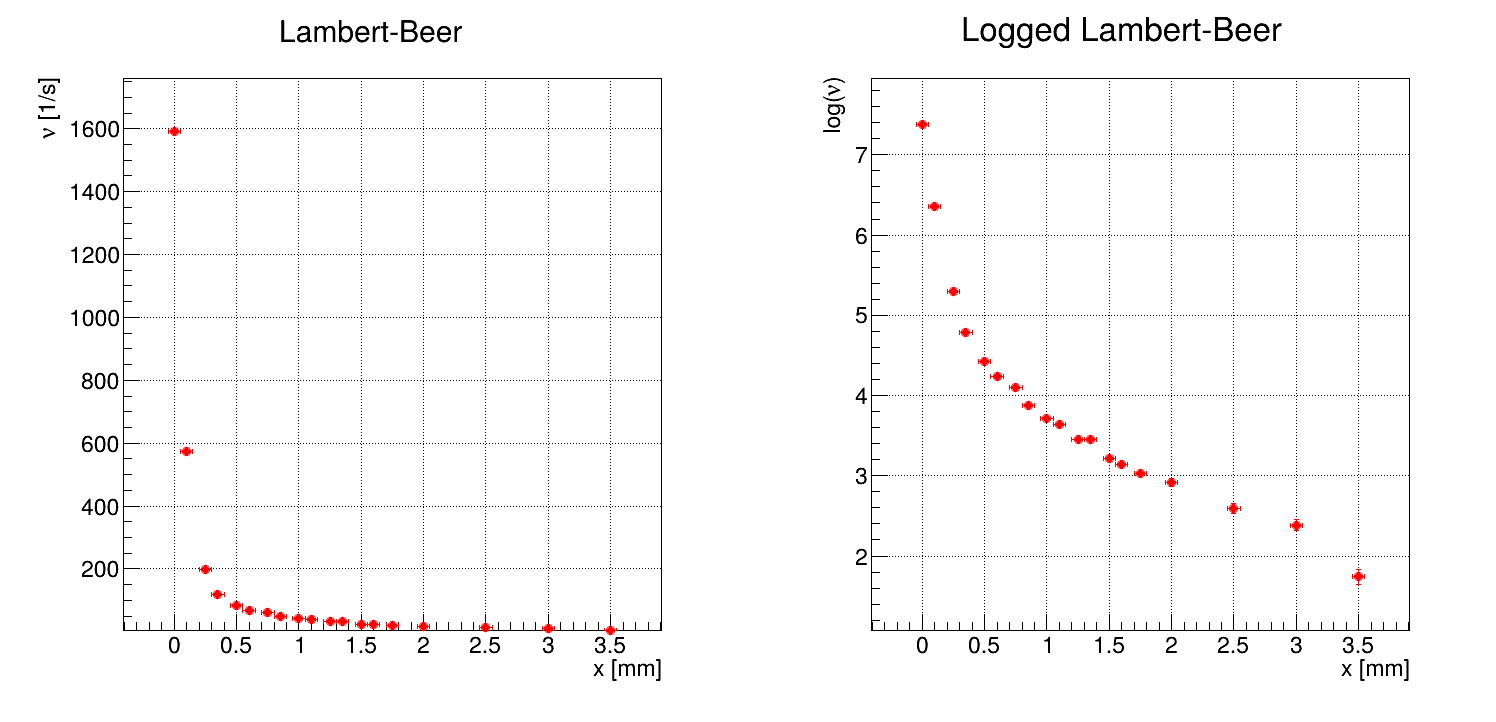
\includegraphics[width=0.8\textwidth]{
figs/CountVsDepthAl.png}
    \caption{Conteggi in funzione della distanza}
    \label{fig:counts-depth}
\end{figure}

Il comportamento atteso dei conteggi in funzione della distanza è una decrescita esponenziale, quindi, in scala logaritmica, una retta. Tuttavia, in figura \cref{fig:counts-depth} l'andamento logaritmico dei conteggi sembra distribuirsi lungo due rette: questo perchè nella legge di Lambert-Beer \cref{eq:lambertbeer} il parametro $\mu$ dipende dall'energia della radiazione.
\\
Assumendo che, per quanto concerne l'assorbimento, lo spettro di emissione sia distribuito attorno a due energie $E_a, E_b$, possiamo riscrivere la legge di decadimento come:
\begin{equation}
  I(x) = I_{0a} e^{-\mu_a x} + I_{0b} e^{-\mu_b x}
\end{equation}
che in scala logaritmica diventa:
\begin{gather}
  \log(I(x)) \big|_a = \log(I_{0a}) - \mu_a x \\
  \log(I(x)) \big|_b = \log(I_{0b}) - \mu_b x
\end{gather}
Nell'ultimo passaggio abbiamo assunto che il logaritmo sia separabile, ovvero, che l'andamento dei conteggi nella zona $a$ non sia significativamente influenzato dall'andamento dei conteggi nella zona b. Questa assunzione è supportata dai dati sperimentali, perchè riconosciamo due rette distinte nel grafico logaritmico

 \help{FORMULE LOGARITMICHE (SORRY NON LE POSSO COPIARE)}

\subsection{Altri effetti}

Qui \ldots

\help{here we talk about the two different behaviours (simo understood it!)}
\help{simo please!}.
